\documentclass[12pt]{article}
 
\usepackage[margin=1in]{geometry}
\usepackage{amsmath,amsthm,amssymb, mathtools}
\usepackage[T1]{fontenc}
\usepackage{lmodern}
\usepackage{fixltx2e}
\usepackage[shortlabels]{enumitem}
\usepackage{mathrsfs}
\usepackage{kbordermatrix}

\usepackage{graphicx}

\renewcommand{\kbldelim}{(}% Left delimiter
\renewcommand{\kbrdelim}{)}% Right delimiter
 
\newcommand{\N}{\mathbb{N}}
\newcommand{\R}{\mathbb{R}}
\newcommand{\Z}{\mathbb{Z}}
\newcommand{\Q}{\mathbb{Q}}
 
\newenvironment{theorem}[2][Theorem]{\begin{trivlist}
\item[\hskip \labelsep {\bfseries #1}\hskip \labelsep {\bfseries #2.}]}{\end{trivlist}}
\newenvironment{lemma}[2][Lemma]{\begin{trivlist}
\item[\hskip \labelsep {\bfseries #1}\hskip \labelsep {\bfseries #2.}]}{\end{trivlist}}
\newenvironment{exercise}[2][Exercise]{\begin{trivlist}
\item[\hskip \labelsep {\bfseries #1}\hskip \labelsep {\bfseries #2.}]}{\end{trivlist}}
\newenvironment{problem}[2][Problem]{\begin{trivlist}
\item[\hskip \labelsep {\bfseries #1}\hskip \labelsep {\bfseries #2.}]}{\end{trivlist}}
\newenvironment{question}[2][Question]{\begin{trivlist}
\item[\hskip \labelsep {\bfseries #1}\hskip \labelsep {\bfseries #2.}]}{\end{trivlist}}
\newenvironment{corollary}[2][Corollary]{\begin{trivlist}
\item[\hskip \labelsep {\bfseries #1}\hskip \labelsep {\bfseries #2.}]}{\end{trivlist}}
\newcommand{\textfrac}[2]{\dfrac{\text{#1}}{\text{#2}}}
\newcommand{\floor}[1]{\left\lfloor #1 \right\rfloor}

\newenvironment{amatrix}[1]{%
  \left(\begin{array}{@{}*{#1}{c}|c@{}}
}{%
  \end{array}\right)
}

\DeclareMathOperator*{\E}{\mathbb{E}}

\newcommand{\Mod}[1]{\ (\mathrm{mod}\ #1)}

\begin{document}

\title{Dynamical Systems: Homework 6}

\author{Chris Hayduk}
\date{December 3, 2020}

\maketitle

\begin{problem}{1}
\end{problem}

The graph for $G = G_A$ is given below,\\
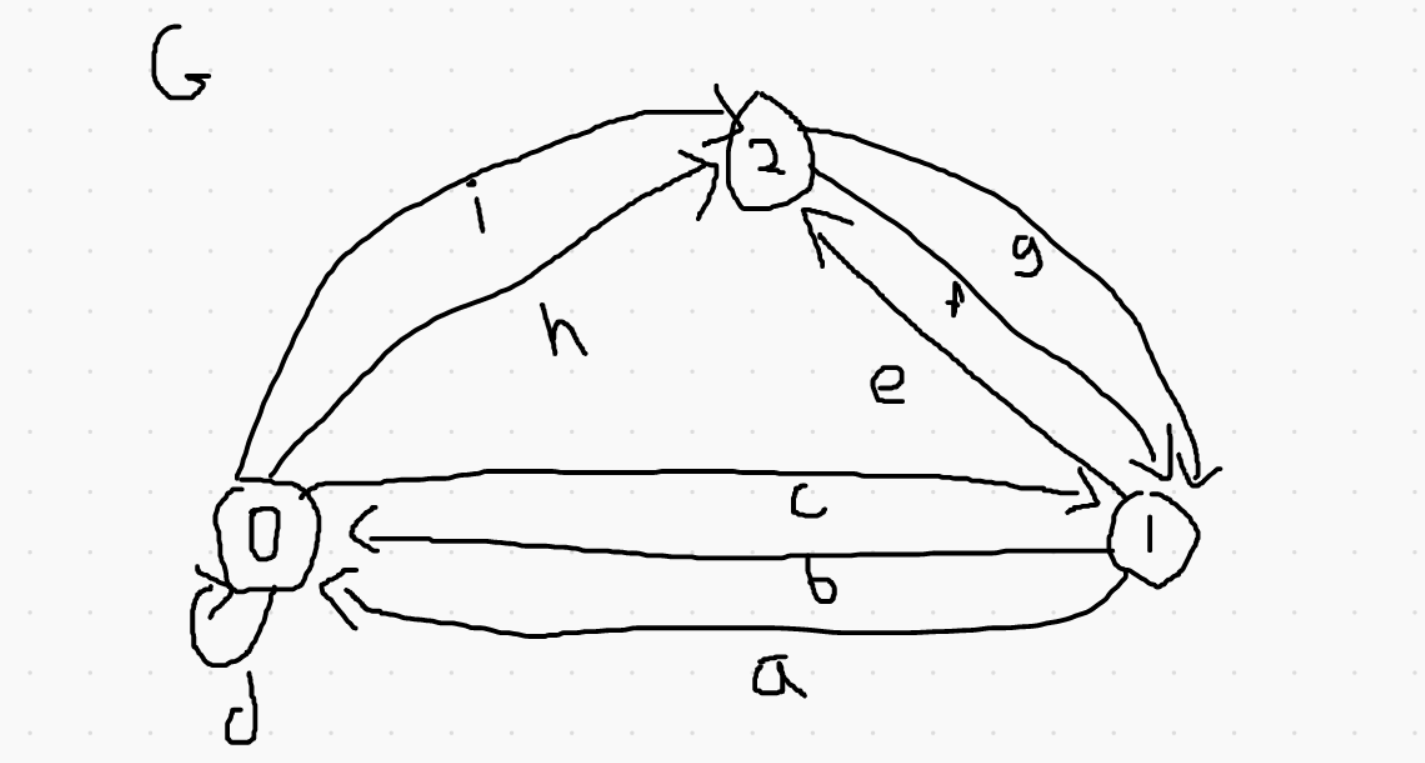
\includegraphics[scale=0.7]{graph.png}

We have labeled the edges above in order to more easily construct the matrix for the shift space, which consists of showing which edges are ``permissible'' following the presence of a given edge. Hence, the shift space, $X$, associated with $G$ is given by the following matrix,
\begin{align*}
X = \kbordermatrix{
    & a & b & c & d & e & f & g & h & i\\
    a & 0 & 0 & 1 & 1 & 0 & 0 & 0 & 1 & 1\\
    b & 0 & 0 & 1 & 1 & 0 & 0 & 0 & 1 & 1\\
    c & 1 & 1 & 0 & 0 & 1 & 0 & 0 & 0 & 0\\
    d & 0 & 0 & 1 & 1 & 0 & 0 & 0 & 1 & 1\\
    e & 0 & 0 & 0 & 0 & 0 & 1 & 1 & 0 & 0\\
    f & 1 & 1 & 0 & 0 & 1 & 0 & 0 & 0 & 0\\
    g & 1 & 1 & 0 & 0 & 1 & 0 & 0 & 0 & 0\\
    h & 0 & 0 & 0 & 0 & 0 & 1 & 1 & 0 & 0\\
    i & 0 & 0 & 0 & 0 & 0 & 1 & 1 & 0 & 0\\
  }
\end{align*}

\begin{problem}{2}
\end{problem}

Define $h: X \to Y$ as $h(00) = 1$, $h(01) = 0$, and $h(10) = 0$. We have defined $h$ over every possible block of size $2$ in the Golden Mean Shift, and each $2$ block has one corresponding size $1$ block in the even shift. Hence, $h$ is a well-defined function from $X \to Y$. Moreover, the pre-image of $0$ in $X$ is $\{01, 10\}$ and the pre-image of $1$ is $\{00\}$. Thus, all of the pre-images are finite so $h$ is finite to one.\\

Now we need to show that $h$ is surjective.

\begin{problem}{3}
\end{problem}

\begin{enumerate}

\item \textbf{Theorem:} Let $(X, d)$ be a compact metric space and let $f: X \to X$ be continuous. If $f$ is transitive and if Per$(f)$ is dense in $X$, then $f$ has sensitive dependence on initial conditions. That is, $f$ is chaotic (since it satisfies all three conditions as stated by Devaney).

This theorem helps to simplify the requirements for $f$ to be choatic, since now we need to only check $2$ conditions rather than $3$.

\item \textbf{Theorem (Sharkovskii's Theorem):} Let $f: \mathbb{R} \to \mathbb{R}$ be continuous with a periodic point of prime period $3$. Then there exist periodic points of any other period.

This results is surprising because of how simply stated, yet powerful it is. We only need to know that $1$ periodic point exists with period $3$ in order to assert that there are periodic points of every other period.

\item \textbf{Theorem:} If $\mathcal{L}$ is a language, then there exists a unique subshift $X$ such that $\mathcal{L}(X) = \mathcal{L}$

In some sense, the subshift $X$ captures all of the information contained in the language.

\item \textbf{Theorem:} $J_{f}$ and $F_{f}$ are completely invariant sets. That is, $f(J_{f}) = J_{f} = f^{-1}(J_{f})$ and $f(F_{f}) = F_{f} = f^{-1}(F_{f})$

Both the Julia set, $J_{f}$, and the Fatou set, $F_{f}$, are closed under the application of $f$ or $f^{-1}$. That is, if we apply $f$ or $f^{-1}$ to any point $x \in J_{f}$, then $f(x), f^{-1}(x) \in J_{f}$. The same holds true for the Fatou set.
\end{enumerate}

\begin{problem}{4}
Bonus problem
\end{problem}

Suppose $X$ is a shift space that is topologically conjugate to a subshit of finite type $Y$. Then there exists a sliding block code $\phi: X \to Y$ such that $\phi$ is invertible.

\end{document}